%%%%%%%%%%%%%%%%%%%%%%%%%%%%%%%%%%%%%%%%%%%%%%%%%%%%%%%%%%%%%%%%%%%%%%%%%%%%
%% Author template for INFORMS Journal on Optimization (ijoo) 
%%   [interim solution; new styles under construction]
%% Mirko Janc, Ph.D., INFORMS, mirko.janc@informs.org
%% ver. 0.93, November 2017
%%%%%%%%%%%%%%%%%%%%%%%%%%%%%%%%%%%%%%%%%%%%%%%%%%%%%%%%%%%%%%%%%%%%%%%%%%%%
\documentclass[ijoo,nonblindrev]{informs-ijoo}

\OneAndAHalfSpacedXI
%%\OneAndAHalfSpacedXII % Current default line spacing
%%\DoubleSpacedXII
%%\DoubleSpacedXI

% Private macros here (check that there is no clash with the style)

% Natbib setup for author-year style
\usepackage{natbib}
 \bibpunct[, ]{(}{)}{,}{a}{}{,}%
 \def\bibfont{\small}%
 \def\bibsep{\smallskipamount}%
 \def\bibhang{24pt}%
 \def\newblock{\ }%
 \def\BIBand{and}%

%% Setup of theorem styles. Outcomment only one.
%% Preferred default is the first option.
\TheoremsNumberedThrough     % Preferred (Theorem 1, Lemma 1, Theorem 2)
%\TheoremsNumberedByChapter  % (Theorem 1.1, Lema 1.1, Theorem 1.2)
\ECRepeatTheorems

%% Setup of the equation numbering system. Outcomment only one.
%% Preferred default is the first option.
\EquationsNumberedThrough    % Default: (1), (2), ...
%\EquationsNumberedBySection % (1.1), (1.2), ...

% For new submissions, leave this number blank.
% For revisions, input the manuscript number assigned by the on-line
% system along with a suffix ".Rx" where x is the revision number.
\MANUSCRIPTNO{MS-0001-1922.65}

%%%%%%%%%%%%%%%%
\begin{document}
%%%%%%%%%%%%%%%%

% Outcomment only when entries are known. Otherwise leave as is and
%   default values will be used.
%\setcounter{page}{1}
%\VOLUME{00}%
%\NO{0}%
%\MONTH{Xxxxx}% (month or a similar seasonal id)
%\YEAR{0000}% e.g., 2005
%\FIRSTPAGE{000}%
%\LASTPAGE{000}%
%\SHORTYEAR{00}% shortened year (two-digit)
%\ISSUE{0000} %
%\LONGFIRSTPAGE{0001} %
%\DOI{10.1287/xxxx.0000.0000}%

% Author's names for the running heads
% Sample depending on the number of authors;
% \RUNAUTHOR{Jones}
\RUNAUTHOR{Slippery and Arinella}
% \RUNAUTHOR{Jones, Miller, and Wilson}
% \RUNAUTHOR{Jones et al.} % for four or more authors
% Enter authors following the given pattern:
%\RUNAUTHOR{}

% Title or shortened title suitable for running heads. Sample:
% \RUNTITLE{Bundling Information Goods of Decreasing Value}
% Enter the (shortened) title:
\RUNTITLE{Tis a Butter Place}

% Full title. Sample:
% \TITLE{Bundling Information Goods of Decreasing Value}
% Enter the full title:
\TITLE{Tis a Far, Far Butter Place}

% Block of authors and their affiliations starts here:
% NOTE: Authors with same affiliation, if the order of authors allows,
%   should be entered in ONE field, separated by a comma.
%   \EMAIL field can be repeated if more than one author
\ARTICLEAUTHORS{%
\AUTHOR{Snidely Slippery}
\AFF{Department of Bread Spread Engineering, Dairy University, Cowtown, IL 60208, \EMAIL{slippery@dairy.edu}} %, \URL{}}
\AUTHOR{Marg Arinella}
\AFF{Institute for Food Adulteration, University of Food Plains, Food Plains, MN 55599, \EMAIL{m.arinella@adult.ufp.edu}}
% Enter all authors
} % end of the block

\ABSTRACT{%
This paper gives an unbelievably detailed history of margarine in
America.  Why then, do you ask, is the title about butter?  Well,
who ever heard of a far, far margarine place?  I mean, come on; you
have to give the author some poetic license.  Otherwise every paper
would read like stereo instructions.  And who ever reads stereo
instructions?  Anyway, the paper is about butter...I mean margarine!
% Enter your abstract
}%

% Sample
%\KEYWORDS{deterministic inventory theory; infinite linear programming duality;
%  existence of optimal policies; semi-Markov decision process; cyclic schedule}

% Fill in data. If unknown, outcomment the field
\KEYWORDS{butter, margarine, silliness} \HISTORY{This paper was
first submitted on April 12, 1922 and has been with the authors for
83 years for 65 revisions.}

\maketitle
%%%%%%%%%%%%%%%%%%%%%%%%%%%%%%%%%%%%%%%%%%%%%%%%%%%%%%%%%%%%%%%%%%%%%%

% Samples of sectioning (and labeling) in MNSC
% NOTE: (1) \section and \subsection do NOT end with a period
%       (2) \subsubsection and lower need end punctuation
%       (3) capitalization is as shown (title style).
%
%\section{Introduction.}\label{intro} %%1.
%\subsection{Duality and the Classical EOQ Problem.}\label{class-EOQ} %% 1.1.
%\subsection{Outline.}\label{outline1} %% 1.2.
%\subsubsection{Cyclic Schedules for the General Deterministic SMDP.}
%  \label{cyclic-schedules} %% 1.2.1
%\section{Problem Description.}\label{problemdescription} %% 2.

% Text of your paper here

\section{Introduction}

Although it has been around for over a century, margarine was not
always the preferred tablespread in the United States. In 1930, per
capita consumption of margarine was only 2.6 pounds (vs. 17.6 pounds
of butter). Times have changed for the better, though (if you're a
margarine manufacturer, that is). Today, per capita consumption of
margarine in the United States is 8.3 pounds (including vegetable
oil spreads) whereas butter consumption is down to about 4.2 pounds.
Furthermore, as shown in Figure \ref{frontier}, it is always butter,
not margarine, that is traded off against guns. This leads to the announcement of our  result.

\begin{theorem}
\label{marg-butt-th}
In a reverse dictionary, $(\mbox{\bi marg}\succ\mbox{\bi butt\/}\; \land\;  
\mbox{\bi arine}\succ\mbox{\bi er})$.
Moreover, continuous reading of a compact subset of the dictionary
attains the minimum of patience at the moment of giving up.
\end{theorem}

The proof will be given in the e-companion to this paper.



\begin{figure}[t]
\begin{center}
\caption{Production Possibilities Frontier.} \label{frontier}
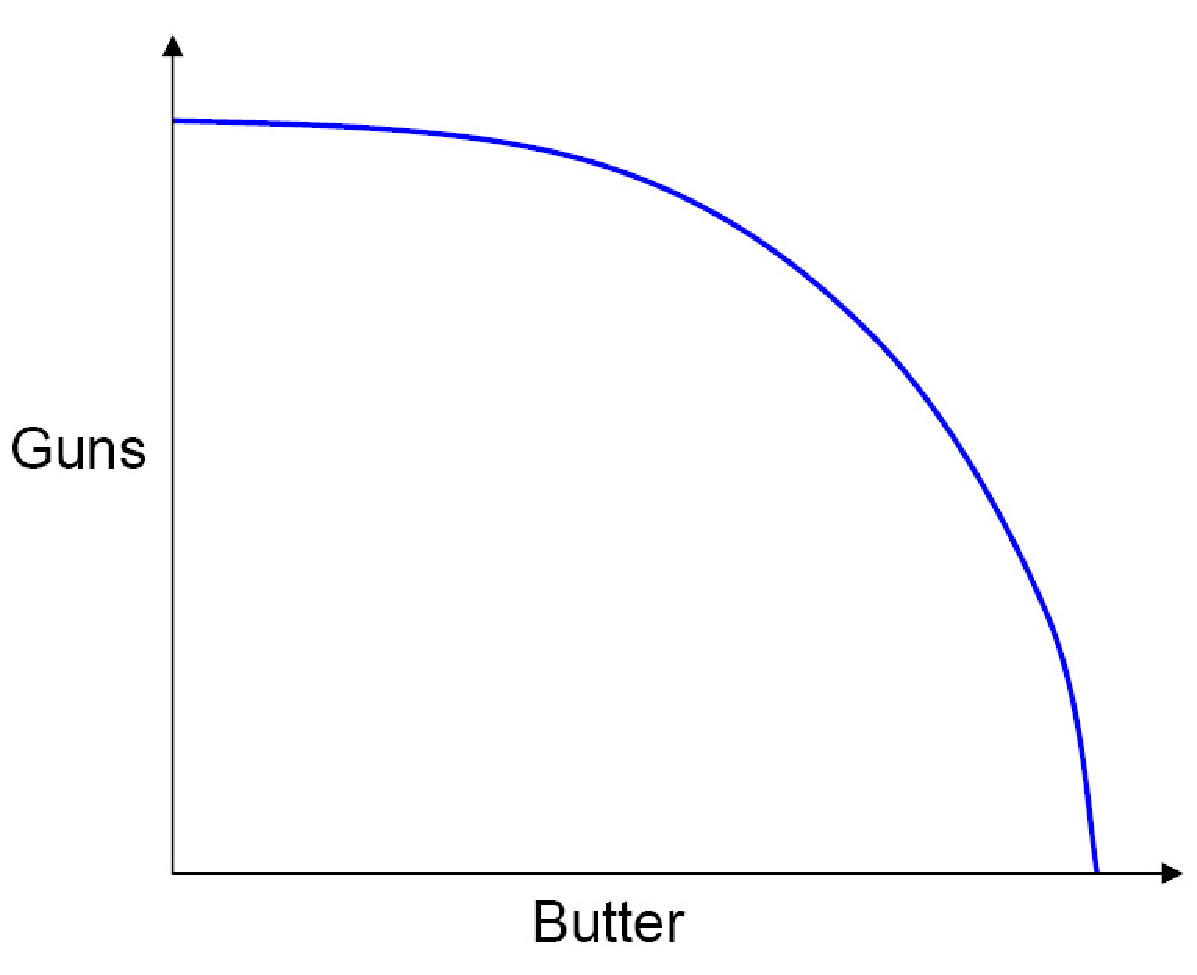
\includegraphics[height=2in]{Sample-Figure.pdf}
\end{center}
\end{figure}

\section{Motivation}

Margarine or butter? According to the website of the 
%%%National Association of Margarine Manufacturers (2005)
\cite{namm}, ``Despite the
recommendations of health professionals and leading health
organizations to choose margarine, many consumers are confused.''
But whether or not they are confused, consumers are voting with
their pocketbooks.  The 
%%%American Butter Institute (2005)
\cite{abi}, whose
slogan is ``Things are better with butter!'', presents many tempting
recipes on its website, but also reports declining sales in its
marketing releases.  

\begin{hypothesis}
Things are better with butter.
\end{hypothesis}

Indeed, even though a reputed chain email letter claims that margarine is ``but 
one molecule from being plastic'' 
%%%(BreakTheChain.org)
\citep{btc}, 
American consumers appear to be
sliding away from butter. Given this trend, a historical review of
margarine is in order.


\begin{lemma}
Many consumers are confused.
\end{lemma}

\begin{lemma}
Whether or not the consumers are confused, they are voting with
their pocketbooks.
\end{lemma}

\begin{proposition}
American consumers are sliding away from butter.
\end{proposition}


\section{Historical Timeline}

The following are milestones in the history of margarine as
reported by the 
%%%National Association of Margarine Manufacturers (2005b)
\cite{namm2}.  
Note that they have been transcribed verbatim here, which
is generally bad practice.  Even if the material is explicitly
indicated as a quotation, having this much content from another
source will almost certainly result in rejection of the paper for
lack of originality.

But if not called out {\em as a quotation}, lifting even a single
sentence (or less) from another source is plagiarism, even if the
source is cited.  Plagiarism is a very serious offense, which will
not only lead to rejection of a paper, but will also bring more
serious sanctions, such as being banned from the journal,
notification of your dean or department chair, etc.  So don't do it!

There are many on-line resources to help determine what constitutes
plagiarism and how to avoid (see, e.g., CollegeBoard.com).  But the
simplest rule to follow is ``when it doubt, call it out.''  That is,
make very plain what comes from other sources, in properly cited
word-for-word quotations or paraphrases.

\section{1800s}

\begin{quotation}

\begin{description}

\item[\bf 1870] Margarine was created by a Frenchman from Provence,
France -- Hippolyte M\`ege-Mouriez -- in response to an offer by
the Emperor Louis Napoleon III for the production of a satisfactory
substitute for butter. To formulate his entry, M\`ege-Mouriez used
margaric acid, a fatty acid component isolated in 1813 by Michael
Chevreul and named because of the lustrous pearly drops that reminded
him of the Greek word for pearl -- margarites. From this word,
M\`ege-Mouriez coined the name margarine for his invention that
claimed the Emperor's prize.

\begin{table}
\TABLE
{All About Marg Arine}
{\begin{tabular}{@{}l@{\qquad}l@{}}
\hline
\up Year&\multicolumn{1}{c}{Margarine milestone\down}\\
\hline\up
1870&Margarine created by Hippolyte M\`ege-Mouriez\\
1873&American patent granted to M\`ege-Mouriez\\
1878&Unilever began manufacturing margarine in Europe\\
1871--1873&U. S. Dairy Company began production of ``artificial butter''\\
1877&State laws requiring identification of margarine passed\\
1881&Improvements to M\`ege-Mouriez's formulation made\\
1885&Congressional passage of the Margarine Act\\
1886&More than 30 manufacturing facilities producing margarine\\
1902&32 states under margarine color bans\\
1902&Tax on colored margarine raised five-fold\down\\
\hline
\end{tabular}}
{}
\end{table}


\item[\bf 1873] An American patent was granted to M\`ege-Mouriez who
intended to expand his French margarine factory and production to
the United States. While demand for margarine was strong in northern
Europe and the potential equally as promising in the U.S.,
M\`ege-Mouriez's operations nevertheless failed and he died obscurely.

\item[\bf 1878] Unilever began manufacturing margarine in Europe.

\item[\bf 1871-73] The U. S. Dairy Company in New York City began
production of "artificial butter."

\item[\bf 1877] State laws requiring identification of margarine were
passed in New York and Maryland as the dairy industry began to feel
the impact of this rapidly growing product

\item[\bf 1881] Improvements to M\`ege-Mouriez's formulation were made;
U.S. Dairy created a subsidiary, the Commercial Manufacturing Company,
to produce several million pounds annually of this new product.

\item[\bf 1885] When a court voided a ban on margarine in New York,
dairy militants turned their attention to Washington, resulting in
Congressional passage of the Margarine Act of 1886. The Act imposed
a tax of two cents per pound on margarine and required expensive
licenses for manufacturers, wholesalers and retailers of margarine.
President Grover Cleveland, from the dairy state of New York, signed
the law, describing it as a revenue measure. However, the 1886 law
failed to slow the sale of margarine principally because it did not
require identification of margarine at the point of sale and
margarine adversaries turned their attention back to the states.

\item[\bf 1886] More than 30 manufacturing facilities were reported to
be engaged in the production of margarine. Among them were Armour
and Company of Chicago and Lever Brothers of New York. Seventeen
states required the product to be specifically identified as
margarine. Various state laws to control margarine were passed in a
number of states, but were not enforced. Later that year, New York
and New Jersey prohibited the manufacture and sale of yellow-colored
margarine.

\end{description}

\end{quotation}



\section{1900s}

\subsection{Before the End of WWII}

\begin{quotation}

\begin{description}

\item[\bf 1902] 32 states and 80\% of the U.S. population lived under
margarine color bans. While the Supreme Court upheld such bans, it
did strike down forced coloration (pink) which had begun in an
effort to get around the ban on yellow coloring. During this period
coloring in the home began, with purveyors providing capsules of
food coloring to be kneaded into the margarine. This practice
continued through World War II.

\item[\bf 1902] Amendments to the Federal Margarine Act raised the tax
on colored margarine five-fold, but decreased licensing fees for
white margarine. But demand for colored margarine remained so
strong, that bootleg colored margarine flourished.

\item[\bf 1904] Margarine production suffered and consumption dropped
from 120 million pounds in 1902 to 48 million.

\item[\bf 1910] Intense pressure by competitors to keep prices low and
new product innovations, as well as dairy price increases, returned
production levels of margarine back to 130 million pounds. The
Federal tax remained despite many efforts to repeal it, but
consumption grew gradually in spite of it.

\item[\bf 1920] With America's entry into World War I, the country began
to experience a fat shortage and a sharp increase in the cost of
living,  both factors in driving margarine consumption to an annual
per capita level of 3.5 pounds.

\item[\bf 1930] The Margarine Act was again amended to place the Federal
tax on naturally-colored (darkened with the use of palm oil) as well
as artificially-colored margarine. During the Depression dairy
interests again prevailed upon the states to enact legislation
equalizing butter and margarine prices. Consumers reacted and
consumption of margarine dropped to an annual per capita level of
1.6 pounds.

\item[\bf 1932] Besides Federal taxes and licenses, 27 states prohibited
the manufacture or sale of colored margarine, 24 imposed some kind
of  consumer tax and 26 required licenses or otherwise restricted
margarine sales. The Army, Navy and other Federal agencies were
barred from using margarine for other than cooking purposes.

\item[\bf 1941] Through production innovations, advertising and improved
packaging, margarine consumption regained lost ground. A Federal
standard  was established recognizing margarine as a spread of its
own kind. With raised awareness of margarine's health benefits from
a 1941 National Nutrition Conference, consumers began to take notice
of restrictions on margarine that were keeping the product from them
and artificially inflating the price.

\item[\bf 1943] State taxes on margarine were repealed in Oklahoma. The courts
removed color barriers in other states shortly after World War II (see \citealt{tjp}).

\end{description}

\end{quotation}


\subsection{After the End of WWII}

\begin{quotation}

\begin{description}


\item[\bf 1947] Residual war shortages of butter sent it to a dollar a pound
and Margarine Act repeal legislation was offered from many politicians.

\item[\bf 1950] Some of the more popular brands prior up until now were Cloverbloom,
Mayflower, Mazola, Nucoa, Blue Plate, Mrs. Filbert's, Parkay,
Imperial, Good  Luck, Nu-Maid, Farmbelle, Shedd's Safflower,
Churngold, Blue Bonnet, Fleischmann's, Sunnyland and Table Maid.

\item[\bf 1950] Margarine taxes and restrictions became the talk of the country.
Finally, following a significant effort by the National Association
of Margarine  Manufacturers, President Truman signed the Margarine
Act of 1950 on March 23 of that year.

\item[\bf 1951] The Federal margarine tax system came to an end. Pre-colored
margarine was enjoyed by a consumer also pleased with lower prices.
Consumption almost doubled in the next twenty years. State color
bans, taxes, licenses and other restrictions began to fall.

\item[\bf 1960s] The first tub margarine and vegetable oil spreads were
introduced to the American public.

\item[\bf 1967] Wisconsin became the last state to repeal restrictions on
margarine \citep{w}.

\item[\bf 1996] A bill introduced by Rep. Ed Whitfield would signal an end
to the last piece of legislation that adversely affects the sale of
margarine. Currently, federal law prohibits the retail sale of
margarine in packages larger than one pound, as well as detailed
requirements regarding the size and types of labeling of margarine
and a color requirement. This new legislation would remove these
restrictions from the Federal Food, Drug, and Cosmetic Act (FFDCA).
Rep. Whitfield's bill, the Margarine Equity Act, is part of HR 3200,
the Food and Drug Administration (FDA) reform package and addresses
dated requirements that are not applicable to the marketplace.

\item[\bf 1998] 125th anniversary of the U.S. patent for margarine

\noindent{{\em Source:} 
%%%National Association of Margarine Manufacturers, 2005
\cite{namm}.}

\end{description}

\end{quotation}



\section{Proof of Theorem \ref{marg-butt-th}.}

To avoid confusion, theorems that we repeat for readers' convenience
will have the same appearance as when they were mentioned for the first
time. However, here they should be coded by \verb+repeattheorem+ instead
of \verb+theorem+ to keep labels/pointers uniquely resolvable. Other predefined theorem-like
environments work similarly if they need to be repeated in what becomes the \mbox{e-companion.}


\begin{repeattheorem}[Theorem 1.]
%\label{marg-butt-th}
In a reverse dictionary, $(\mbox{\bi marg}\succ\mbox{\bi butt\/}\; \land\;  
\mbox{\bi arine}\succ\mbox{\bi er})$.
Moreover, continuous reading of a compact subset of the dictionary
attains the minimum of patience at the moment of giving up.
\end{repeattheorem}

\subsection{Preparatory Material}

\begin{lemma}
\label{aux-lem1}
In a reverse dictionary, $\mbox{\bi g}\succ\mbox{\bi t\/}$.
\end{lemma}

\begin{lemma}
\label{aux-lem2}
In a reverse dictionary, $\mbox{\bi e}\succ\mbox{\bi r\/}$.
\end{lemma}

\proof{Proof of Lemmas \ref{aux-lem1} and \ref{aux-lem2}.} See the alphabet and the tebahpla.\Halmos
\endproof

\begin{remark} 
Note that the title of the proof should be keyed
explicitly in each case. Authors can hardly agree on what would be the
default proof title, so there is no default. Even \verb+\proof{Proof.}+ should be keyed out. 
\end{remark}


\subsection{Proof of the Main Result}

\proof{Proof of Theorem 1.} The first statement is a conseqence of
Lemma~\ref{aux-lem1} and \ref{aux-lem2}. The rest relies on the fact that the continuous
image of a compact set into the reals is a closed interval, thus having
a minimum point.\Halmos 
\endproof

\begin{figure}[t]
\begin{center}
\caption{Production Possibilities Frontier Again.} \label{ECfrontier}
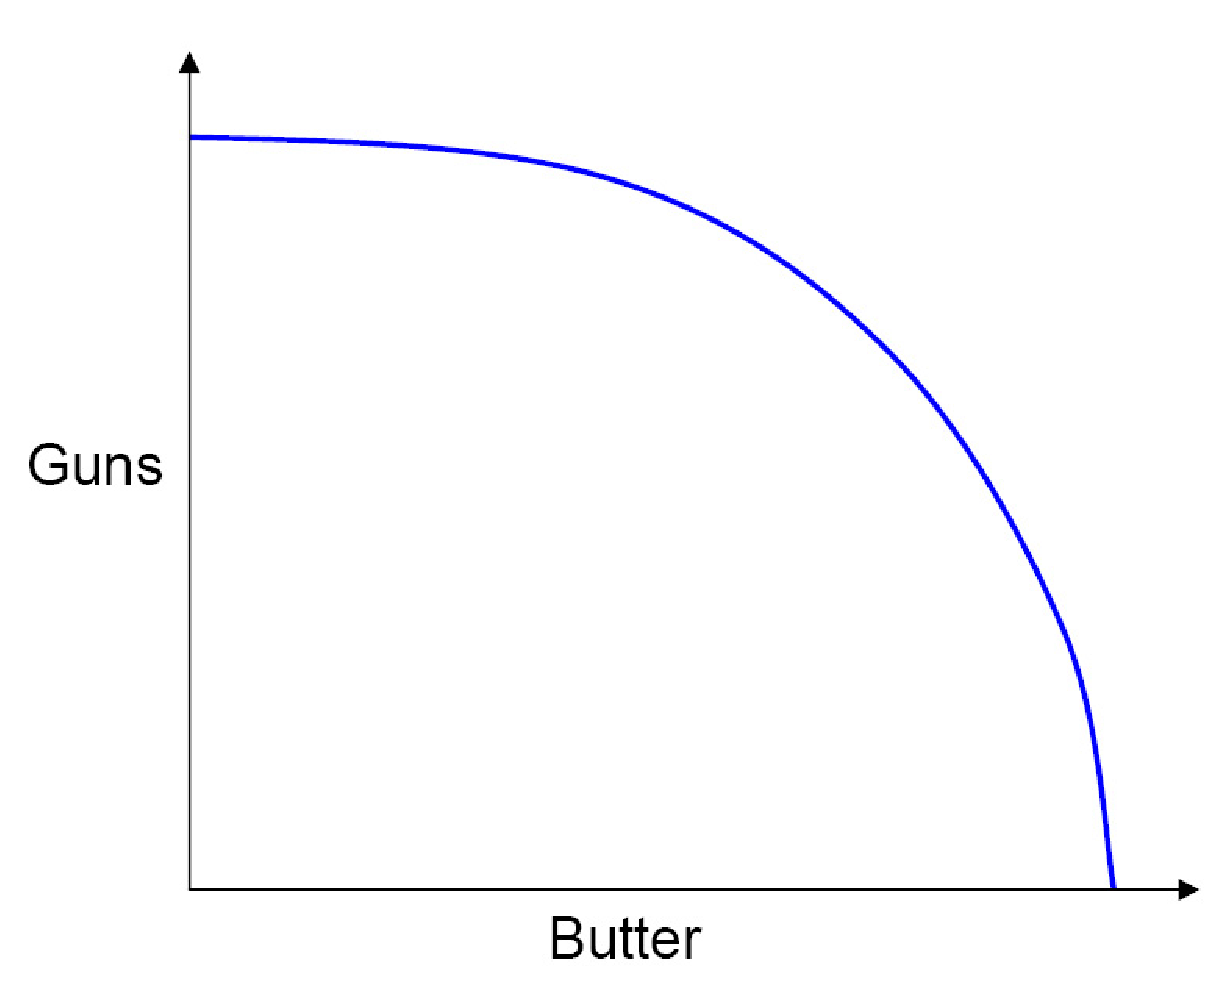
\includegraphics[height=1.5in]{Sample-Figure}
\end{center}
\end{figure}



\section{Conclusions}

Since we didn't do anything original in this paper, we don't
actually have any conclusions.  But we have to have a conclusions
section in here, so we're writing one.  Don't the margins look good?
How about those section headings?  Pretty snappy, eh?

However, just because we didn't produce any results, doesn't mean
that there isn't good butter re-search going on out there.  Many
researchers 
%%%(e.g., Tholstrup et al. 2006, Hodson et al. 2001)
(e.g., \citealt{trbn}, \citealt{h})
continue to push out the envelope of our understanding of butter and
its health effects.  Others are focusing on related products, such as cheese 
%%%(see, e.g., Fontecha et al. 2006).  
(see, e.g., \citealt{fo}).  
Still others are
investigating the linguistic 
%%%(Feldman and Schwan 1990) 
\citep{fs}
and sociopolitical 
%%%(Geisel 1984) 
\citep{g}
implications of butter.  So butter
remains a hot research area with lots of potential for the future.

All the potential in the world won't amount to much if research
isn't cited correctly, though. Make sure you include complete
citation information for your references, including publication or
re-trieval dates for website citations, publication year and volume
and issue numbers for journal articles, publisher names and
locations for books, reports, and conference proceedings, and page
numbers for eve-rything, but especially for direct quotes. For
citations of unpublished work, you need to include the date of
update, as well as the name and address of the organization that
sponsored the work. Take a look at the reference section below to
see how references should be formatted.


% Appendix here
% Options are (1) APPENDIX (with or without general title) or
%             (2) APPENDICES (if it has more than one unrelated sections)
% Outcomment the appropriate case if necessary
%
% \begin{APPENDIX}{<Title of the Appendix>}
% \end{APPENDIX}
%
%   or
%
% \begin{APPENDICES}
% \section{<Title of Section A>}
% \section{<Title of Section B>}
% etc
% \end{APPENDICES}


% Acknowledgments here
\ACKNOWLEDGMENT{The authors gratefully acknowledge the existence of
the Journal of Irreproducible Results and the support of the Society
for the Preservation of Inane Research.}


% References here (outcomment the appropriate case)

% CASE 1: BiBTeX used to constantly update the references
%   (while the paper is being written).
%\bibliographystyle{informs2014} % outcomment this and next line in Case 1
%\bibliography{<your bib file(s)>} % if more than one, comma separated

% CASE 2: BiBTeX used to generate mypaper.bbl (to be further fine tuned)
%\input{mypaper.bbl} % outcomment this line in Case 2

%If you don't use BiBTex, you can manually itemize references as shown below.


\bibliographystyle{nonumber}

\begin{thebibliography}{}

\bibitem[{American Butter Institute(2005)}]{abi}
American Butter Institute (2005) Dairy market report. Retrieved June
14, 2005, www.butterinstitute.org.

\bibitem[{BreakTheChain.org(2005)}]{btc}
BreakTheChain.org (2005) Is butter better? Retrieved June 14, 2005,
http://www.breakthechain.org/\penalty0{}exclusives/margarine.html.

\bibitem[{CollegeBoard.com(2005)}]{cb}
CollegeBoard.com (2005)  How to avoid plagiarism. Retrieved June 14,
2005,
http://www.collegeboard.\penalty0{}com/article/0,3868,2-10-0-10314,00.html.

\bibitem[{Feldman and Schwan(1990)}]{fs}
Feldman D, Schwan K (1990) {\it Who Put the Butter in Butterfly
and Other Fearless Investigations into Our Illogical Language}
(HarperPerennial, New York).

\bibitem[{Fontecha et~al.(2006)}]{fo}
Fontecha J, Mayo I, Toledano G, Juarez M (2006)
Triacylglycerol composition  of projected designation
of origin cheeses during ripening. {\it J. Dairy Sci.} 89:882--887.

\bibitem[{Geisel(1984)}]{g}
Geisel TS (1984) {\it The Butter Battle Book}  (Random House, New York).

\bibitem[{Hodson et~al.(2001)}]{h}
Hodson L, Skeaff CM, Chisholm W-AH (2001) The effect of
replacing dietary saturated fat with polyunsaturated or
monounsaturated fat on plasma lipids in free-living young adults.
{\it Eur. J. Clinical Nutrition} 55(10):908--915.

\bibitem[{National Association of Margarine Manufacturers(2005a)}]{namm}
National Association of Margarine Manufacturers (2005a) Margarine in
the news. Retrieved June 14, 2005, www.margarine.org. 

\bibitem[{National Association of Margarine Manufacturers(2005b)}]{namm2}
National Association of Margarine Manufacturers (2005b) Margarine in
the news. Retrieved Termidor 1, 1790, www.margarine.org.

\bibitem[{www.margarine.org(2005)}]{hist}
The History of Margarine (2005) 
www.margarine.org/historyofmargarine.html. Retrieved June 14. 

\bibitem[{Tholstrup et al.(2006)}]{trbn} 
Tholstrup T, Raff M, Basu S, Nonboe P, Sejrsen K, Staarup EM (2006) 
Effects of butter and monounsaturated fatty acids
into lipid classes, plasma C-reactive protein, oxidative stress,
hemostatic variables, and insulin in healthy young men. {\it Amer. J.
Clinical Nutrition} 83:237--243.

\bibitem[{Torbica et al.(2006)}]{tjp}
Torbica A, Jovanovic O, Pajin B (2006) The advantages of solid
fat content determination in cocoa butter and cocoa butter
equivalents by the Karlshamns method. {\it Eur. Food Res. Techn.} {\bf 222}
385--391.

\bibitem[{Williams(1994)}]{w}
Williams BR (1994) {\it The Best Butter in the World: A History of
Sainsbury's} (Ebury Press, London).

\end{thebibliography}

%%%%%%%%%%%%%%%%%
\end{document}
%%%%%%%%%%%%%%%%%

